\begin{titlepage}
    \centering
    \vspace*{1.5cm}
    
    {\scshape\LARGE AstDyn Project \par}
    \vspace{1cm}
    
    \rule{\linewidth}{0.5mm} \\[0.4cm]
    {\Huge\bfseries Scientific Reference Manual \par}
    \vspace{0.4cm} 
    \rule{\linewidth}{0.5mm} \\[1.5cm]
    
    {\Large\textit{High-Fidelity C++ Library for Asteroid Dynamics\\and Occultation Prediction} \par}
    
    \vspace{2cm}
    
    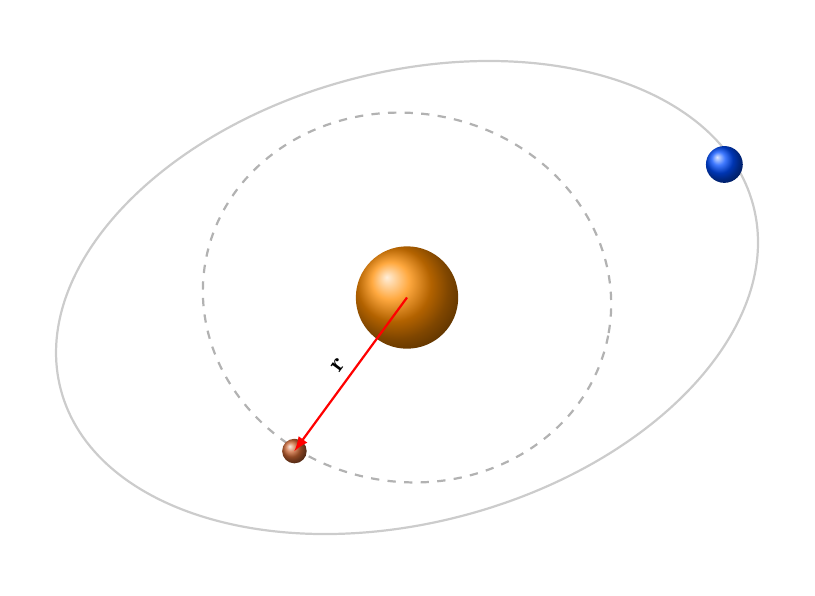
\begin{tikzpicture}[scale=1.3]
        % Abstract representation of solar system dynamics
        % Sun
        \shade[ball color=orange!90!yellow] (0,0) circle (0.5);
        
        % Orbits
        \draw[gray!40, thick, rotate=15] (0,0) ellipse (3.5 and 2.2);
        \draw[gray!60, thick, dashed, rotate=-10] (0,0) ellipse (2.0 and 1.8);
        
        % Bodies
        \shade[ball color=blue!70!cyan] (3.1, 1.3) circle (0.18); % Earth-like
        \shade[ball color=brown!80!red] (-1.1, -1.5) circle (0.12); % Asteroid
        
        % Vector annotation (symbolic)
        \draw[->, >=latex, red, thick] (0,0) -- node[above, sloped, black] {\small $\mathbf{r}$} (-1.1, -1.5);
    \end{tikzpicture}
    
    \vspace{2.5cm}
    
    \begin{minipage}{0.4\textwidth}
        \begin{flushleft} \large
        \emph{Author:}\\
        Michele \textsc{Bigi}
        \end{flushleft}
    \end{minipage}
    \begin{minipage}{0.4\textwidth}
        \begin{flushright} \large
        \emph{Version:}\\
        1.0.0 \\
        \vspace{0.2cm}
        \emph{Date:}\\
        \today
        \end{flushright}
    \end{minipage}
    
    \vfill
    
    {\large \textit{Validated against JPL DE441 Ephemerides}}
    
    \vspace{1.5cm}
\end{titlepage}
\clearpage
